% !TEX encoding = UTF-8 Unicode
\documentclass{sig-alternate}
\usepackage{textcomp}
\usepackage{graphics}
\usepackage[utf8]{inputenc}
\usepackage[T1]{fontenc}

\hyphenation{li-neal co-rrec-ci\'on pro-ble-ma Back-propagation con-si-de-ra}

\begin{document}

\pagenumbering{arabic}

\title{Algoritmos Genéticos}
\subtitle{Sistemas de Inteligencia Artificial - ITBA}

\numberofauthors{3}

\author{
	\alignauthor{Carlos Sessa}\\
	\alignauthor{Lucas Pizzagalli}\\
	\alignauthor{Nicolás Purita}\\	
}

\date{12 de Junio de 2012}

\maketitle

\section*{Introducción}

	Se implementó un algoritmo genético para obtener los pesos para la red neuronal construida en el TP2.
	La red neuronal resuelve una función con la siguiente forma:

	\begin{figure}[!ht]
		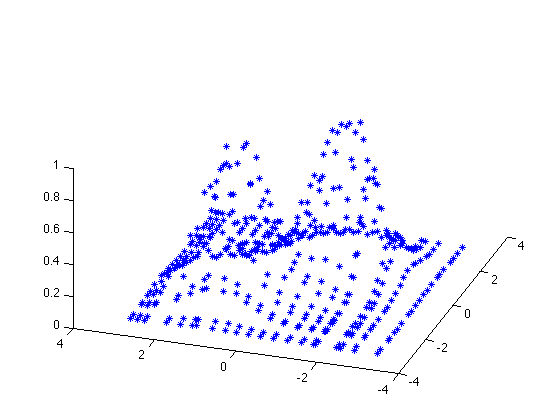
\includegraphics[scale=0.5]{./figures/function.png}
  		\caption{Distribución de puntos dada}
  		\label{fig:function}
	\end{figure}

	En la figura \ref{fig:function} se puede observar que los puntos de la entrada pertenecen al intervalo $[-3.5, 3.5]$ y la salida se encuentra en el intervalo $(0, 1)$.\\
	El algoritmo genético se implementó en \textit{Java} y la red neuronal fue realizada en \textit{Matlab}.
	Utilizando el \textit{MATLAB Compiler Runtime} se prueban los pesos obtenidos en la red.

\section*{Desarrollo y Problemas encontrados}

Completar
	
\section*{Resultados y Conclusiones}

Completar


\end{document}
